\begin{center}

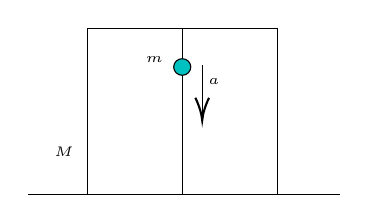
\begin{tikzpicture}[x=0.75pt,y=0.75pt,yscale=-1,xscale=1]
%uncomment if require: \path (0,300); %set diagram left start at 0, and has height of 300

%Shape: Rectangle [id:dp9922461305951003] 
\draw   (178.4,60) -- (270,60) -- (270,140) -- (178.4,140) -- cycle ;
%Straight Lines [id:da3301501137208056] 
\draw    (224.2,60) -- (224.2,140) ;
%Shape: Ellipse [id:dp5458618741603067] 
\draw  [color={rgb, 255:red, 0; green, 0; blue, 0 }  ,draw opacity=1 ][fill={rgb, 255:red, 0; green, 192; blue, 192 }  ,fill opacity=1 ] (220.08,78.67) .. controls (220.08,76.46) and (221.93,74.67) .. (224.2,74.67) .. controls (226.48,74.67) and (228.32,76.46) .. (228.32,78.67) .. controls (228.32,80.88) and (226.48,82.67) .. (224.2,82.67) .. controls (221.93,82.67) and (220.08,80.88) .. (220.08,78.67) -- cycle ;
%Straight Lines [id:da7738101207130361] 
\draw    (233.82,77.78) -- (233.82,102.44) ;
\draw [shift={(233.82,104.44)}, rotate = 270] [color={rgb, 255:red, 0; green, 0; blue, 0 }  ][line width=0.75]    (10.93,-3.29) .. controls (6.95,-1.4) and (3.31,-0.3) .. (0,0) .. controls (3.31,0.3) and (6.95,1.4) .. (10.93,3.29)   ;
%Straight Lines [id:da09431715141860386] 
\draw    (150,140) -- (300,140) ;

% Text Node
\draw (161.37,116.17) node [anchor=north west][inner sep=0.75pt]  [font=\tiny] [align=left] {$\displaystyle M$};
% Text Node
\draw (205.42,72.61) node [anchor=north west][inner sep=0.75pt]  [font=\tiny] [align=left] {$\displaystyle m$};
% Text Node
\draw (235.65,82.83) node [anchor=north west][inner sep=0.75pt]  [font=\tiny] [align=left] {$\displaystyle a$};


\end{tikzpicture}

\end{center}